\section{10 класс}

% Задача 19, Задачи факультатива, относительность движения
\begin{wrapfigure}{r}{3.5cm}
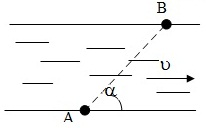
\includegraphics[width=3.5cm]{0115RelativityPowerboats.jpg}
\end{wrapfigure}

\AddProb Два катера вышли одновременно из пунктов $A$ и $B$, находящихся на противоположных берегах реки и расположенных на расстоянии~$L$, 
двигаясь по прямой~$AB$. Прямая $AB$ образует угол $\alpha$ с направлением скорости течения~$v$. Скорости движения катеров относительно воды одинаковы. 
На каком расстоянии от пункта $B$ произошла встреча катеров, если они встретились через время $\tau$ после отхода от причалов.

\AddProb Шарик массы $m$ подвешен на идеальной пружине жесткости~$k$, имеющей начальную длину~$L_0$, над центром платформы центробежной машины. 
Шарик начинает вращаться с угловой скоростью~$\omega$. Какой угол образует при этом пружина с вертикалью? 
Проанализируйте зависимость угла отклонения пружины от параметров задачи.

\AddProb Для измерения температуры $t$ собрана схема, состоящая из четырех резисторов, подключенная к источнику с ЭДС $U$ и малым внутренним сопротивлением. 
Температурные коэффициенты сопротивления резисторов попарно равны и составляют соответственно $\alpha_1$ и~$\alpha_2$, 
а сопротивления всех резисторов при температуре $0^{\circ}C$ одинаковы. Как зависит напряжение между точками $1$ и $2$ от температуры? 
Считать, что в диапазоне измеряемых температур $\alpha_1t<<1$, $\alpha_2t<<1$.

\AddProb Найти зависимость от времени силы~$F$, действующей на дно цилиндрического стакана площади~$S$, в который из чайника с высоты~$H$ 
наливают воду плотности~$\rho$. Известно, что каждую секунду в стакан наливают одинаковый объем воды, равный~$Q$.



\section{11 класс}

% Задача 19, Задачи факультатива, относительность движения
\begin{wrapfigure}{r}{3.5cm}
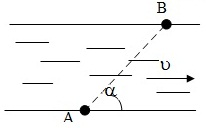
\includegraphics[width=3.5cm]{0115RelativityPowerboats.jpg}
\end{wrapfigure}

\AddProb Два катера вышли одновременно из пунктов $A$ и $B$, находящихся на противоположных берегах реки и расположенных на расстоянии~$L$, 
двигаясь по прямой~$AB$. Прямая $AB$ образует угол $\alpha$ с направлением скорости течения~$v$. Скорости движения катеров относительно воды одинаковы. 
На каком расстоянии от пункта $B$ произошла встреча катеров, если они встретились через время $\tau$ после отхода от причалов.

\AddProb Шарик массы $m$ подвешен на идеальной пружине жесткости~$k$, имеющей начальную длину~$L_0$, над центром платформы центробежной машины. 
Шарик начинает вращаться с угловой скоростью~$\omega$. Какой угол образует при этом пружина с вертикалью? 
Проанализируйте зависимость угла отклонения пружины от параметров задачи.

\AddProb Для измерения температуры $t$ собрана схема, состоящая из четырех резисторов, подключенная к источнику с ЭДС $U$ и малым внутренним сопротивлением. 
Температурные коэффициенты сопротивления резисторов попарно равны и составляют соответственно $\alpha_1$ и~$\alpha_2$, 
а сопротивления всех резисторов при температуре $0^{\circ}C$ одинаковы. Как зависит напряжение между точками $1$ и $2$ от температуры? 
Считать, что в диапазоне измеряемых температур $\alpha_1t<<1$, $\alpha_2t<<1$.

\AddProb На рисунке показан циклический процесс для $\nu$ молей гелия, состоящий из двух участков линейной зависимости давления $p$ от объема $V$ 
и одной изобары. Известно, что на изобаре $3 - 1$ над газом была совершена работа $A$ $(A > 0)$, а температура газа уменьшилась в $n\,=\,4$ раза. 
Точки $2$ и $3$ лежат на одной изотерме. Точки $1$ и $2$ на диаграмме $pV$ лежат на прямой, проходящей через начало координат. 
Определите температуру газа в точке $1$ и работу газа за весь цикл.